\chapter{Introducion} \label{ch:Introduction}
\section{Interferon-Induced Proteins with Tetratricopeptide Repeats} \label{sec:Interferon-Induced Proteins with Tetratricopeptide Repeats}
The interferon-induced proteins with tetratricopeptide repeats (\textit{IFIT}) gene family are interferon-stimulated genes (ISGs) that are activated early in antiviral response. In unstimulated cells, with the exception of some myeloid cell subsets, they are barely detectable; however, upon viral infection their translated products become some of the most abundant proteins in the cell (\cite{Diamond2013TheProteins}). \textit{IFITs} are conserved in higher animals yet absent in the genomes of plants, insect, and yeast. 

With regards to their genomic composition, they are composed of two exons, the first encoding the ATG, two additional nucleotides and a 5’ untranslated region (UTR), with the second exon containing the rest of the coding sequence and 3’UTR (\cite{deVeer1998IFI60/ISG60/IFIT4Genes}). Most of the IFIT family gene members contain multiple copies of specific sequences in their promoter regions called interferon-stimulated response elements (IRSE), which are targets for downstream effectors of the interferon signalling cascade, enabling the fast activation of IFIT gene transcription (\cite{Lou2009Ifr-9/stat2Stat1}).   

Most mammalian IFIT genes are categorised into 4 subgroups named IFIT1, IFIT2, IFIT3, and IFIT5 all with clear orthologous relationships (\cite{Sarkar2004NovelGenes}). Primates, along with some other mammalian species have a duplication of IFIT1 called IFIT1B, which lacks the ISRE in its gene promoter regions. Several rodents including mice and rats have lost the IFIT1 and IFIT5 genes and have duplications of IFIT1B and IFIT3 (\cite{Daugherty2016Evolution-guidedMammals.}) resulting in IFIT1B (typically referred to as IFIT1), IFIT1B-like gene 1, IFIT1B-like 2 gene, IFIT3 and IFIT3B genes. In contrast, avian species have lost most IFIT genes, with only one left resembling human IFIT5 (\cite{Liu2013Lineage-SpecificFamily}). These variations in IFIT gene numbers are most probably the result of differing evolutionary pressures posed by different viruses affecting their respective host species, although it is evident that maintaining IFIT genes in the genome must be beneficial. 




\subsection{Routes of \textit{IFIT} Expression Activation} \label{subsec:Routes of IFIT Expression Activation}
\subsubsection{Interferon Signalling} \label{Interferon Signalling}
\textit{IFIT} induction can be achieved by activating several arms of the innate immune system (Figure \ref{fig:Pathways Inducing ISG mRNA Production.}). The strongest inducers are type I interferons, such as Interferon alpha and beta (IFN\(\alpha\)/\(\beta\)).  Their signalling is mediated via activation of IFN\(\alpha\)/\(\beta\) receptor and the subsequent downstream Janus kinase (JAK), and Signal transducer and activator of transcription (STAT) signal transduction. As a result, interferon-stimulated gene factor 3 (ISGF3), consisting of phosphorylated STAT1 and STAT2 proteins bound to interferon regulatory factor (IRF) IRF9, translocates to the nucleus, binds to the ISRE in the IFIT promoters and induces their transcription (\cite{Der1998IdentificationArrays}; \cite{Mesev2019DecodingInfection}; \cite{Schoggins2011Interferon-stimulatedFunctions}). 




\subsubsection{Pattern Recognition Receptors} \label{Pattern Recognition Receptors}
Another arm of \textit{IFIT} activation is mediated through several pattern recognition receptors (PRRs), which can recognise various pathogen-associated molecular patterns (PAMPs). \textit{IFITs} have been reported to be induced by bacterial PAMPs such as lipopolysaccharide (LPS) from Neisseria meningitidis via activation of Toll-like receptor (TLR) 4 (\cite{Zhou2013InterferonDefense.}). Interestingly, TLR4 has also been observed to be activated by the glycoprotein of respiratory syncytial virus (RSV) (\cite{Funchal2015RespiratoryNeutrophils}). Other TLRs such as TLR3, TLR7, and TLR9 are capable of sensing PAMPs in the form of foreign nucleic acids in the endosomes. TLRs then interact with their adaptor proteins to in turn activate IRF3, IRF7, and nuclear factor kappa B (NF\(\kappa\)B), all of which have the capability to induce \textit{IFIT} family genes (\cite{Diamond2013TheProteins}). These pathways are often prevalent in lymphocytes, monocytes, and mast cells; however, cytosolic nucleic acid sensors are functional in a broader subset of cells (\cite{Ablasser2011WhereFit}).

\begin{figure}
    \centering
    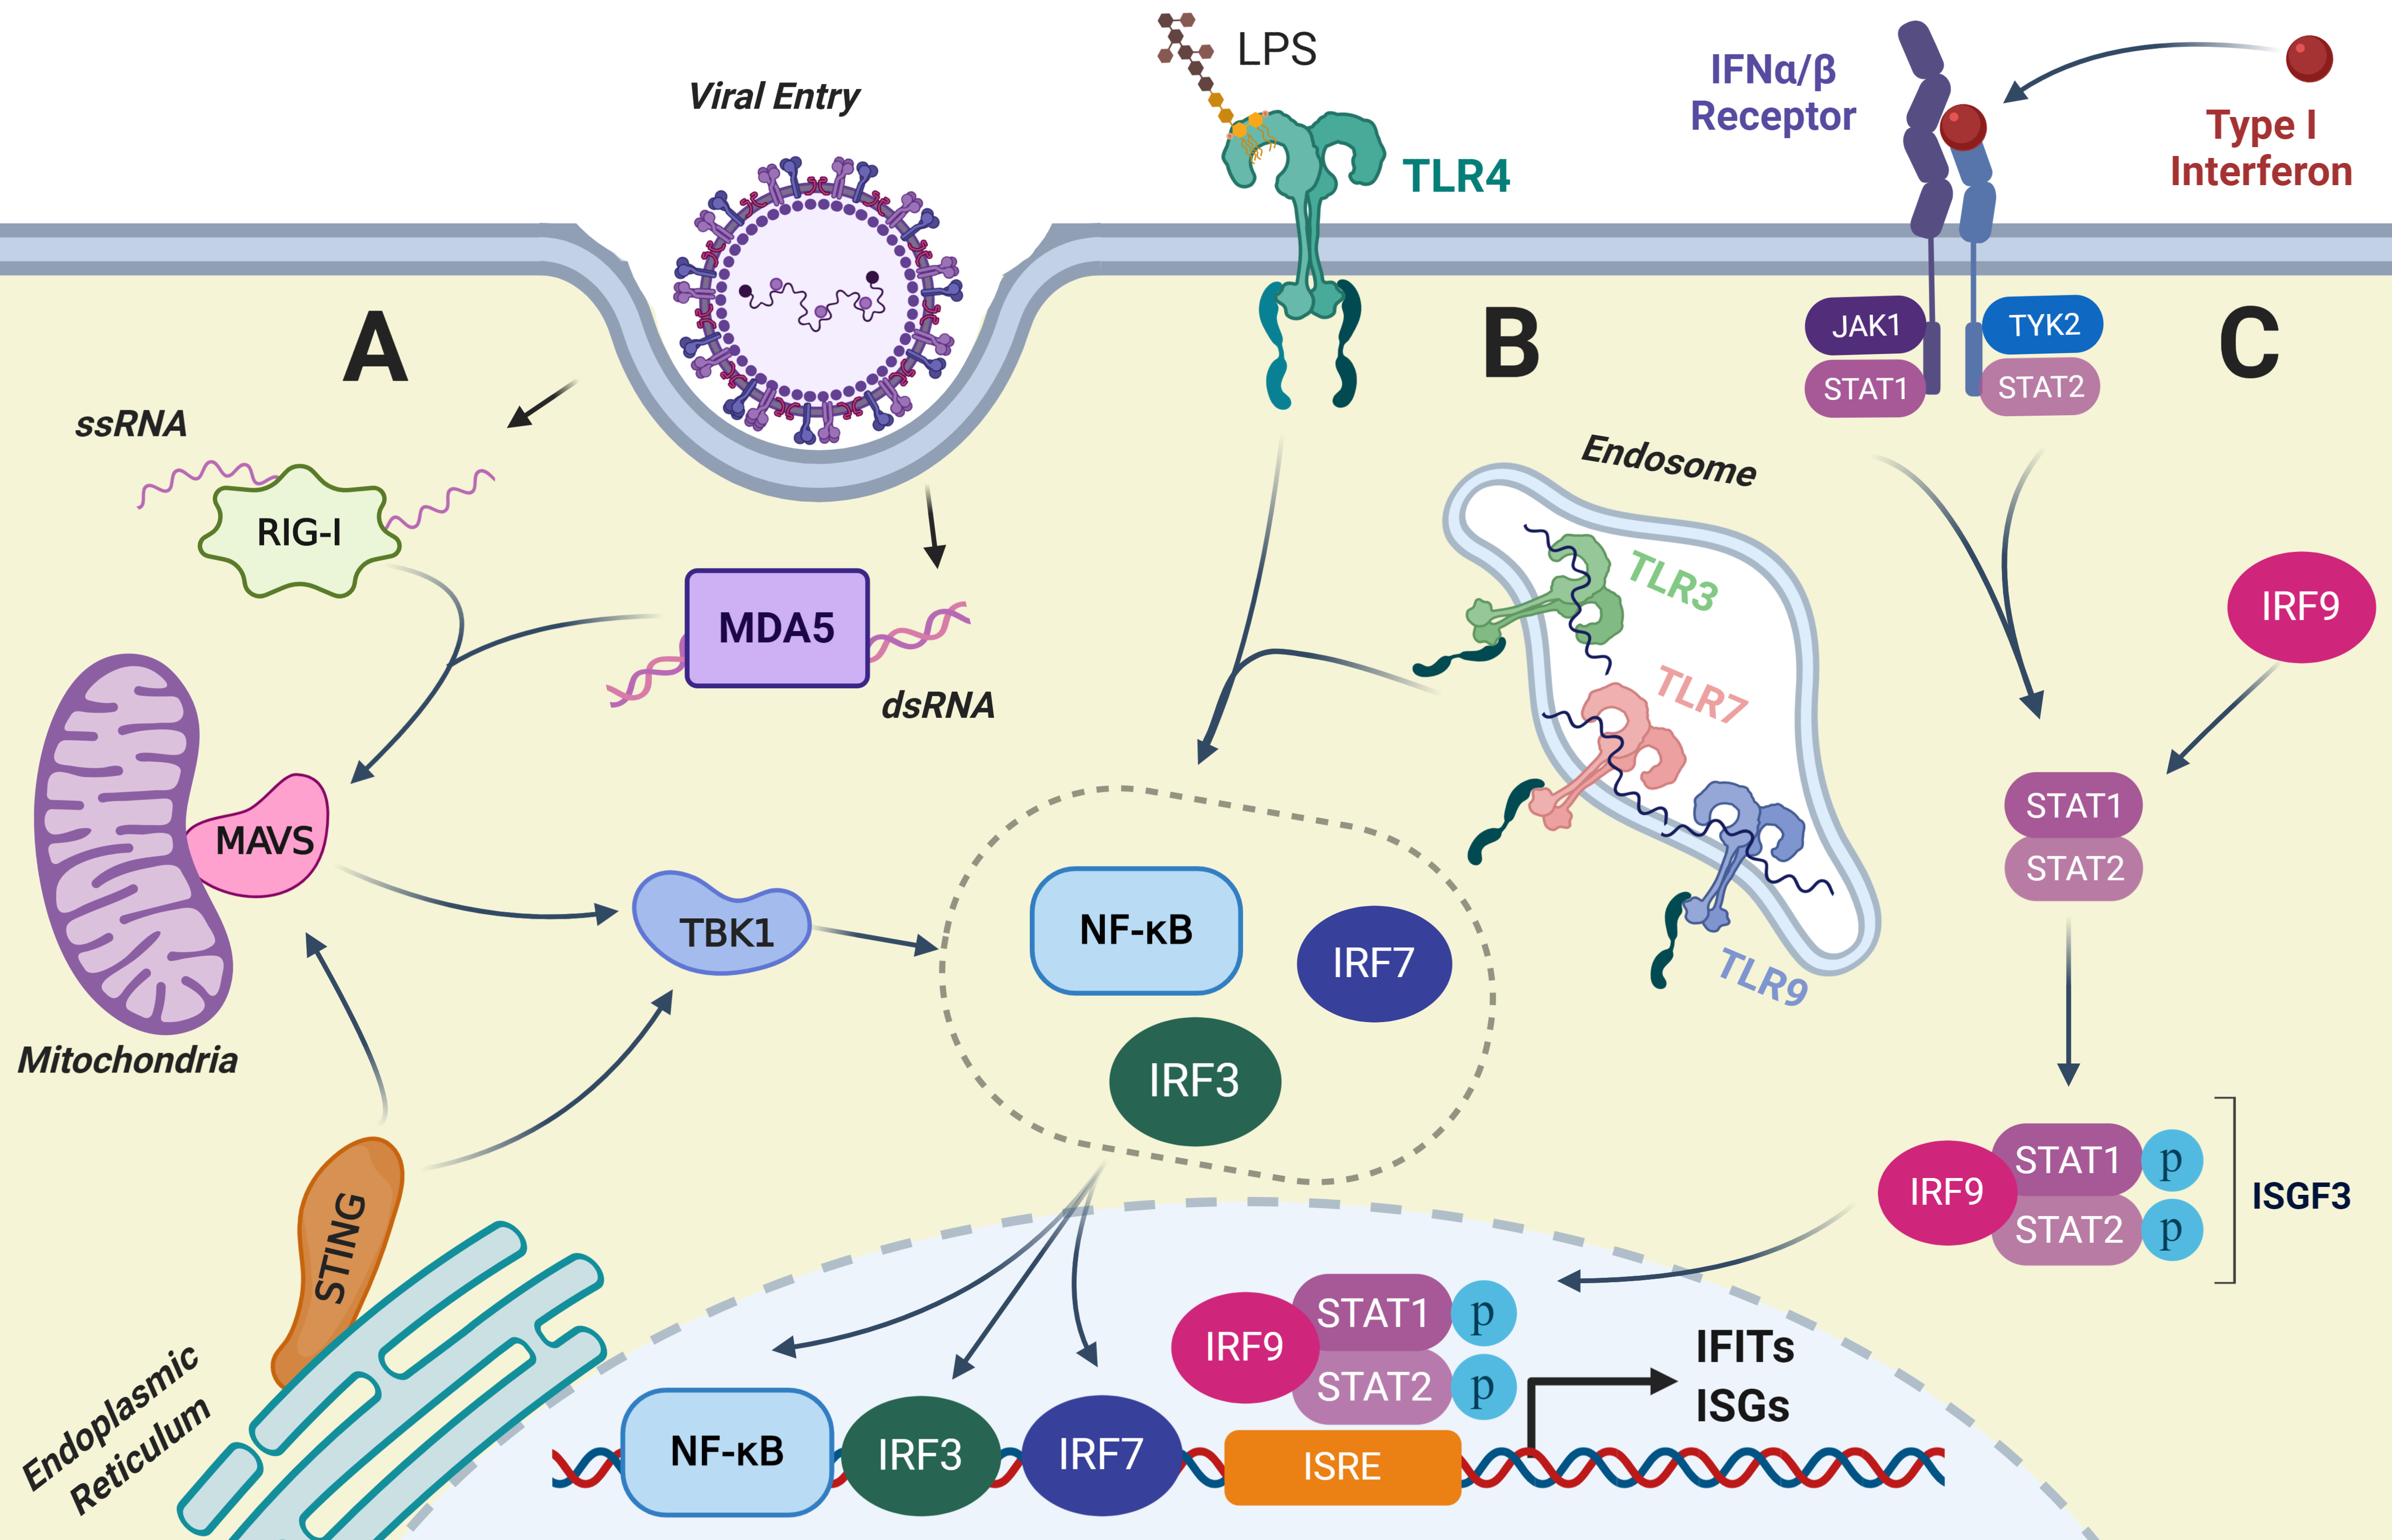
\includegraphics[width=1\linewidth]{04. Introduction//Figs/01. IFIT transcription activation figure.png}
    \caption[Pathways Inducing ISG mRNA Production.]{\textbf{Pathways Inducing ISG mRNA Production.} Three routes of ISGs transcription induction are depicted. Pathway A shows virus releasing its genome upon its entry and subsequent foreign nucleic acid detection by cytosolic sensors RIG-I and MDA5. These detect single-stranded and double-stranded RNA respectively. Both activate MAVS, which in turn activates TBK1. STING protein facilitates this activation by enhancing MAVS and TBK1 interaction. Pathway B shows PAMP detection by TLR receptors. TLR4 recognises LPS in the extracellular space while TLR3, TLR7, and TLR9 detect foreign nucleic acids in endosomes. TBK1, as well as TLR activation, leads to translocation of activated IRF3, IRF7, and NF\(\kappa\)B into the nucleus where they promote ISGs transcription activation. Pathway C depicts type 1 interferon signalling pathway. IFN\(\alpha\)/\(\beta\) receptor activation leads to STAT1 and STAT2 activation. Further addition of IRF9 forms ISGF3 complex, which translocates into the nucleus onto ISRE and promotes ISGs transcription activation. ISG, interferon-stimulated genes; RIG-I, retinoic acid-inducible gene-I; MDA5, melanoma differentiation-associated gene 5; MAVS, mitochondrial antiviral signalling protein; TBK1, TANK-binding kinase 1; STING, stimulator of interferon genes; PAMP, pathogen-associated molecular pattern; TLR, toll-like receptor; IRF, interferon regulatory factor; NF\(\kappa\)B, nuclear factor kappa B; IFN, interferon; STAT, signal transducer and activator of transcription; ssRNA, single-stranded RNA; dsRNA, double-stranded RNA; ISGF, interferon-stimulated gene factor; ISRE, interferon-stimulated response elements. The figure was adapted from Diamond and Farzan, (2013) and Natalya Odoardi’s BioRender template. Created with BioRender.com.}
    \label{fig:Pathways Inducing ISG mRNA Production.}
\end{figure}




\subsubsection{Cytosolic Nuclec Acid Sensors} \label{Cytosolic Nuclec Acid Sensors}
Cytosolic RNA sensors include melanoma differentiation-associated gene 5 (MDA5) and retinoic acid-inducible gene I (RIG-I) (\cite{Vladimer2014IFITs:Proteins}). Both signal through mitochondrial antiviral signalling protein (MAVS), which in turn activates IRF3, IRF7, and NF\(\kappa\)B as their downstream effectors (\cite{Ashley2019Interferon-IndependentCytomegalovirus}). In order to prevent activation by cellular RNA molecules, a precise RNA-recognition mechanism has to be conducted by the sensors. While MDA5 senses long double-stranded RNA (dsRNA) (\cite{Brisse2019ComparativeMDA5.}), RIG-I is able to sense differences in the 5’ RNA modifications (\cite{Schlee2016DiscriminatingSensing}). During mRNA maturation in higher eukaryotes, 7-methyl guanosine (m7G) is connected by a 5’- 5’ triphosphate bridge, which is referred to as capping (\cite{Devarkar2016StructuralRIG-I}; \cite{Ramanathan2016MRNAApplications}). Several viruses carry uncapped, 5’-triphosphorylated (5’-PPP) or incompletely capped RNA (cap 0), whereas host animals possess cap-1 and cap-2 mRNA moieties (\cite{Choi2018ACaps}), which are all depicted in Figure \ref{fig:Overview of 5'RNA Modifications.}. \textit{IFITs} can be activated by several signal transduction pathways, each with its own inducers and kinetics. A cross-play of these pathways is what in turn orchestrates IFIT response during viral infection.

\begin{figure}
    \centering
    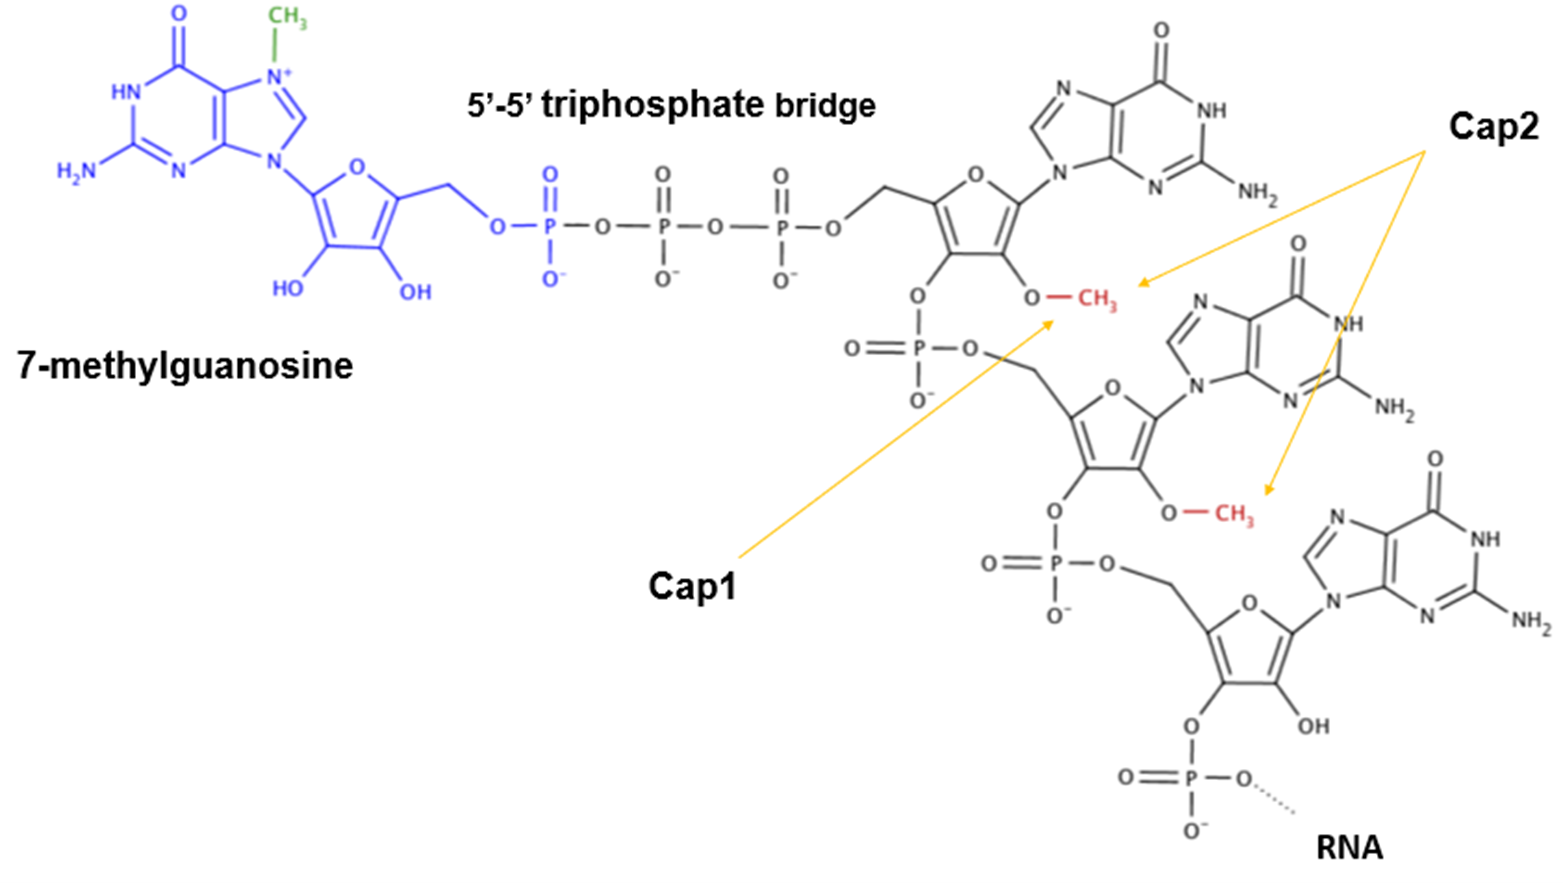
\includegraphics[width=0.75\linewidth]{04. Introduction//Figs/02. 5-RNA Modifications.png}
    \caption[Overview of 5'RNA Modifications.]{\textbf{Overview of 5'RNA Modifications.} Mature mRNA is displayed. Higher eukaryotes modify their mRNA by the initial addition of guanosine (blue) via 5’ - 5’ triphosphate bridge to the 5’ end. Subsequently, the guanosine is methylated into 7-methylguanosine (green) and this modification is referred to as Cap0 structure. Furthermore, the first 2 bases of RNA can be methylated (red) and make either Cap1 or Cap2 structural modification (yellow arrows). The figure was adapted from \cite{Picard-Jean2013RNAGenomes}.}
    \label{fig:Overview of 5'RNA Modifications.}
\end{figure}




\subsection{Structural Features of IFIT Proteins} \label{subsec:Structural Features of IFIT Proteins}
IFITs are composed of multiple copies of tetratricopeptide repeats (TPR). These are motifs comprised of 3-16 tandem repeats of 34 amino acids, which adopt helix-turn-helix confirmations (\cite{DAndrea2003TPRHelix}). TPRs are conserved in all species from bacteria through plants to higher animals and are commonly found in scaffolding proteins (\cite{Vladimer2014IFITs:Proteins}). IFIT TPRs are comprised of degenerate sequences meaning the conservation of the motif is limited. This allows different IFIT proteins to have a broader profile of protein interactors while still maintaining the overall conformation (\cite{Fensterl2015Interferon-InducedPathogenesis}). IFIT proteins are often subjected to post-translational modifications such as ubiquitination or ISGylation (addition of small IFN-induced ubiquitin-like proteins), which may alter IFIT stability and function.




\subsubsection{IFITs Act as Non-Self RNA Sensors} \label{IFITs Act as Non-Self RNA Sensors}
IFIT1 and IFIT5 both form a positively charged channel with an affinity for 5’ ends of single-stranded RNA (ssRNA) molecules in a sequence non-specific manner. IFIT5 can accommodate 5’PPP RNA and effectively acts as a sensor for these molecules (\cite{Abbas2013StructuralProteins}; \cite{Pichlmair2011IFIT1RNA}). On the other hand, IFIT1 can accommodate m7G, but certain residues inside its channel prevent efficient binding of cap1 and cap2 moieties (\cite{Diamond2014IFIT1:Translation}; \cite{Mears2018BetterResponse}). 

PUT MORE ON IFIT2!! PUT MORE ON IFIT2!! PUT MORE ON IFIT2!! PUT MORE ON IFIT2!! PUT MORE ON IFIT2!! PUT MORE ON IFIT2!! 

\begin{figure}
    \centering
    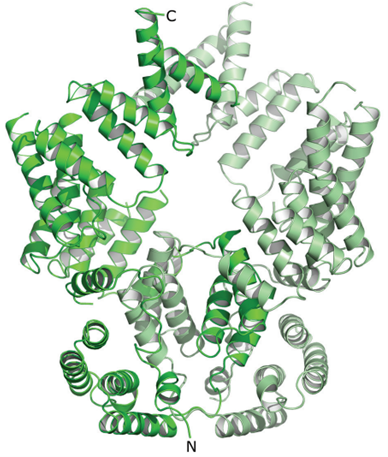
\includegraphics[width=0.25\linewidth]{04. Introduction//Figs/03. IFIT2-structure.png}
    
    
\end{figure}

\begin{figure}
    \centering
    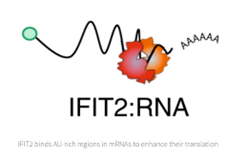
\includegraphics[width=0.25\linewidth]{04. Introduction//Figs/04. IFIT2-rna-binding.png}
    
    
\end{figure}




\subsubsection{Formation of IFIT Protein Complexes} \label{Formation of IFIT Protein Complexes}
As shown in Figure \ref{fig:IFIT Structures and Multimer Formation.}, all IFIT proteins, apart from IFIT5, can form homo- and hetero- dimeric and trimeric complexes. IFIT1 homodimerizes via its C-terminal domain (\cite{Abbas2013StructuralProteins}). The same domain has been shown to interact with the C termini of both IFIT2 and IFIT3, although the IFIT1:IFIT3 complex is more thermodynamically stable (\cite{Fleith2018IFIT3RNA}). Compared to IFIT1, IFIT5 has its dimerization motif shielded by its C terminal TPR and thus stays monomeric in solution (\cite{Kumar2014InhibitionMRNAs}). In contrast, IFIT2 and IFIT3 are rarely seen as monomeric in solution and rather stay as their respective homodimers or IFIT2:3 heterodimers. This is predicted to be done by swapping the third TRP domain in their N-terminal domains (Figure \ref{fig:IFIT Structures and Multimer Formation.}), which keeps them in a more thermodynamically stable configuration (\cite{Yang2012CrystalMechanisms}). IFIT2 homodimer forms a large positively charged cavity which has a propensity to bind dsRNA and AU-rich RNA molecules (\cite{Vladimer2014IFITs:Proteins}; \cite{Yang2012CrystalMechanisms}). IFIT3 interacts with IFIT1 via its C-terminal domain and this interaction increases the half-life of IFIT1 and its specificity for cap0 RNA. Thus, IFIT3 acts as an enhancer of IFIT1 action (\cite{Fleith2018IFIT3RNA}; \cite{Johnson2018HumanStability}). Recently, it has been shown that IFIT1, IFIT2, and IFIT3 form a heterotrimer, although the precise function of this complex has yet to be elucidated (\cite{Fleith2018IFIT3RNA}). In summary, TPR motifs allow IFITs to have a multitude of possible interaction partners, including themselves. Formation of IFIT homo- and hetero-oligomers influences their function and half-life, allowing for variable possible outcomes to occur following IFIT protein production based on the level of each of the proteins. 

\begin{figure}
    \centering
    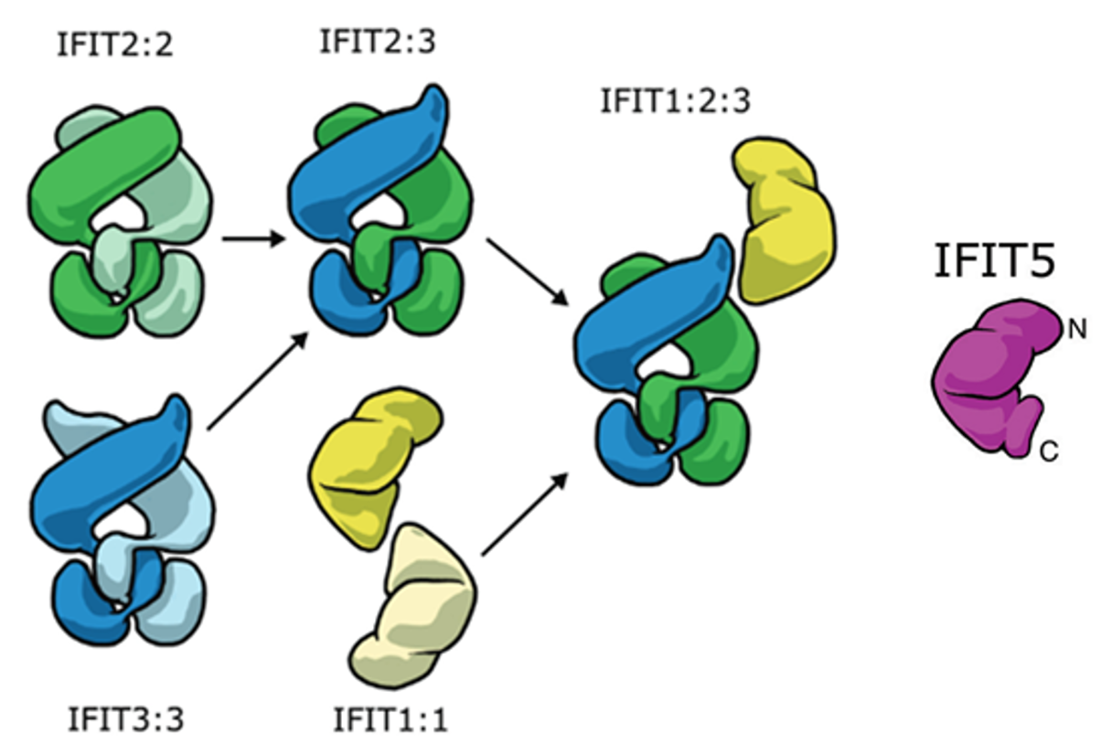
\includegraphics[width=0.75\linewidth]{04. Introduction//Figs/05. IFIT-complexes.png}
    \caption[IFIT Structures and Multimer Formation.]{\textbf{IFIT Structures and Multimer Formation.} IFIT tertiary and quaternary protein conformations are illustrated. IFIT1 is shown in yellow, IFIT2 in green, IFIT3 in blue, and IFIT5 is highlighted in purple. IFIT1 is able to homodimerise or heterooligomerise with IFIT2 and IFIT3 via its C terminal domain. IFIT5 has the corresponding interaction domain occluded by a helix and thus does not interact with the rest of IFIT proteins. IFIT2 and IFIT3 are capable of forming homodimers or heterodimers by ‘swapping’ TPRs in their N terminal regions. By combining the interactions IFIT1:2:3 heterotrimer is formed. The figure was adapted from \cite{Mears2018BetterResponse}.}
    \label{fig:IFIT Structures and Multimer Formation.}
\end{figure}




\subsection{Functions of IFIT Proteins} \label{subsec:Functions of IFIT Proteins}
\subsubsection{Inhibition of Translation and Viral Replication} \label{Inhibition of Translation and Viral Replication}
IFITs can restrict viral replication by several mechanisms. IFIT1 and IFIT5 can physically prevent non-self RNA from interacting with eukaryotic initiation factor (eIF) 4F (\cite{Kumar2014InhibitionMRNAs}). IFIT1 and 2 block the binding of eIF3 to the eIF2–GTP–Met-tRNA ternary complex by interacting with the eIF3E subunit, whereas human IFIT2, and mouse IFIT1 and IFIT2, can block the formation of the 43S–mRNA complex by binding to the eIF3C subunit (\cite{Diamond2014IFIT1:Translation}; \cite{Guo2000CharacterizationVirus}). This is a cap-independent mechanism for viral translation inhibition, however, extensive IFIT expression can negatively influence the whole cellular translation processes via this mechanism and can hinder normal inflammatory responses. Overexpression of IFIT1 in human embryonic kidney (HEK) 293T cells inhibited the activation of IRF3 and NF\(\kappa\)B and the transcription of IFN\(\beta\) in response to polyinosinic–polycytidylic acid (poly I:C) (\cite{Li2009ISG56Response}). The previously mentioned affinity of IFIT2 for AU-rich RNA can also regulate cellular translation as a lot of transcripts for cytokines or apoptotic factors are rich in adenine and uracil (\cite{Palanisamy2012ControlMicroRNAs}). 




\subsubsection{Modulation of Innate Immune Response Signalling} \label{Modulation of Innate Immune Response Signalling}
IFIT proteins also have the potential to influence innate immune responses by direct interaction with signalling cascade proteins. IFIT3 can potentiate RIG-I signalling by forming a scaffold between MAVS and TANK-binding kinase 1 (TBK1), (\cite{Liu2011IFN-InducedTBK1}), whereas IFIT5 enhances this pathway upstream by recruiting RIG-I to MAVS (\cite{Zhang2013IFIT5Pathways}). IFIT5 has also been reported to help facilitate NF\(\kappa\)B activation via scaffolding its activation kinases (\cite{Zhang2013IFIT5Pathways}). On the other hand, studies show that IFIT1 can both negatively and positively influence RIG-I signalling, upstream of MAVS. IFIT1 interacts with the stimulator of interferon genes (STING), an enhancer of MAVS and TBK1 interaction and it was proposed that these conflicting actions are caused by its multiple binding sites on STING (\cite{Li2009ISG56Response}; \cite{Reynaud2015IFIT1Interferon}). 




\subsubsection{Effects on Cell Cycle Progression and Apoptosis} \label{Effects on Cell Cycle Progression and Apoptosis}
IFIT2 and IFIT3 also have roles in cellular homeostasis. IFIT2 overexpression induces the mitochondrial-dependant apoptotic pathway. IFIT2 has been shown to localise on mitochondrial membranes and to directly interact with pro-apoptotic factors which leads to apoptosome formation and subsequent caspase-9 activation (\cite{Chen2017InhibitionApoptosis}; \cite{Diamond2013TheProteins}). Expression of IFIT3 has been observed to alleviate these effects, most probably by the formation of IFIT2:3 dimers (\cite{Mears2018BetterResponse}; \cite{Stawowczyk2011TheApoptosis}). IFIT3 has also been observed to have negative effects on proliferation via indirect degradation of cyclin-dependant kinase inhibitor p27. As a result, cell cycle progression halts at G1/S transition checkpoint (\cite{Xiao2006RIG-GProteins}). An overview of the IFIT mechanisms of action is depicted in Figure \ref{fig:Overview of IFIT Mechanisms of Action}.

Therefore, IFITs not only act as complementary RNA sensors to RIG-I but are also important as mediators of a plethora of other processes. These range from regulation of transcription, activation and inhibition of innate immune signalling, and regulation of cell life cycle. It is again possible that preference for these actions is influenced by the levels of particular IFIT proteins and their interplay. Taking into consideration the above-described modes of IFIT expression activation, we can speculate that different stimuli such as viruses or signalling molecules at different concentrations will result in quite diverging actions of IFIT proteins on the phenotype of the cell.

\begin{figure}
    \centering
    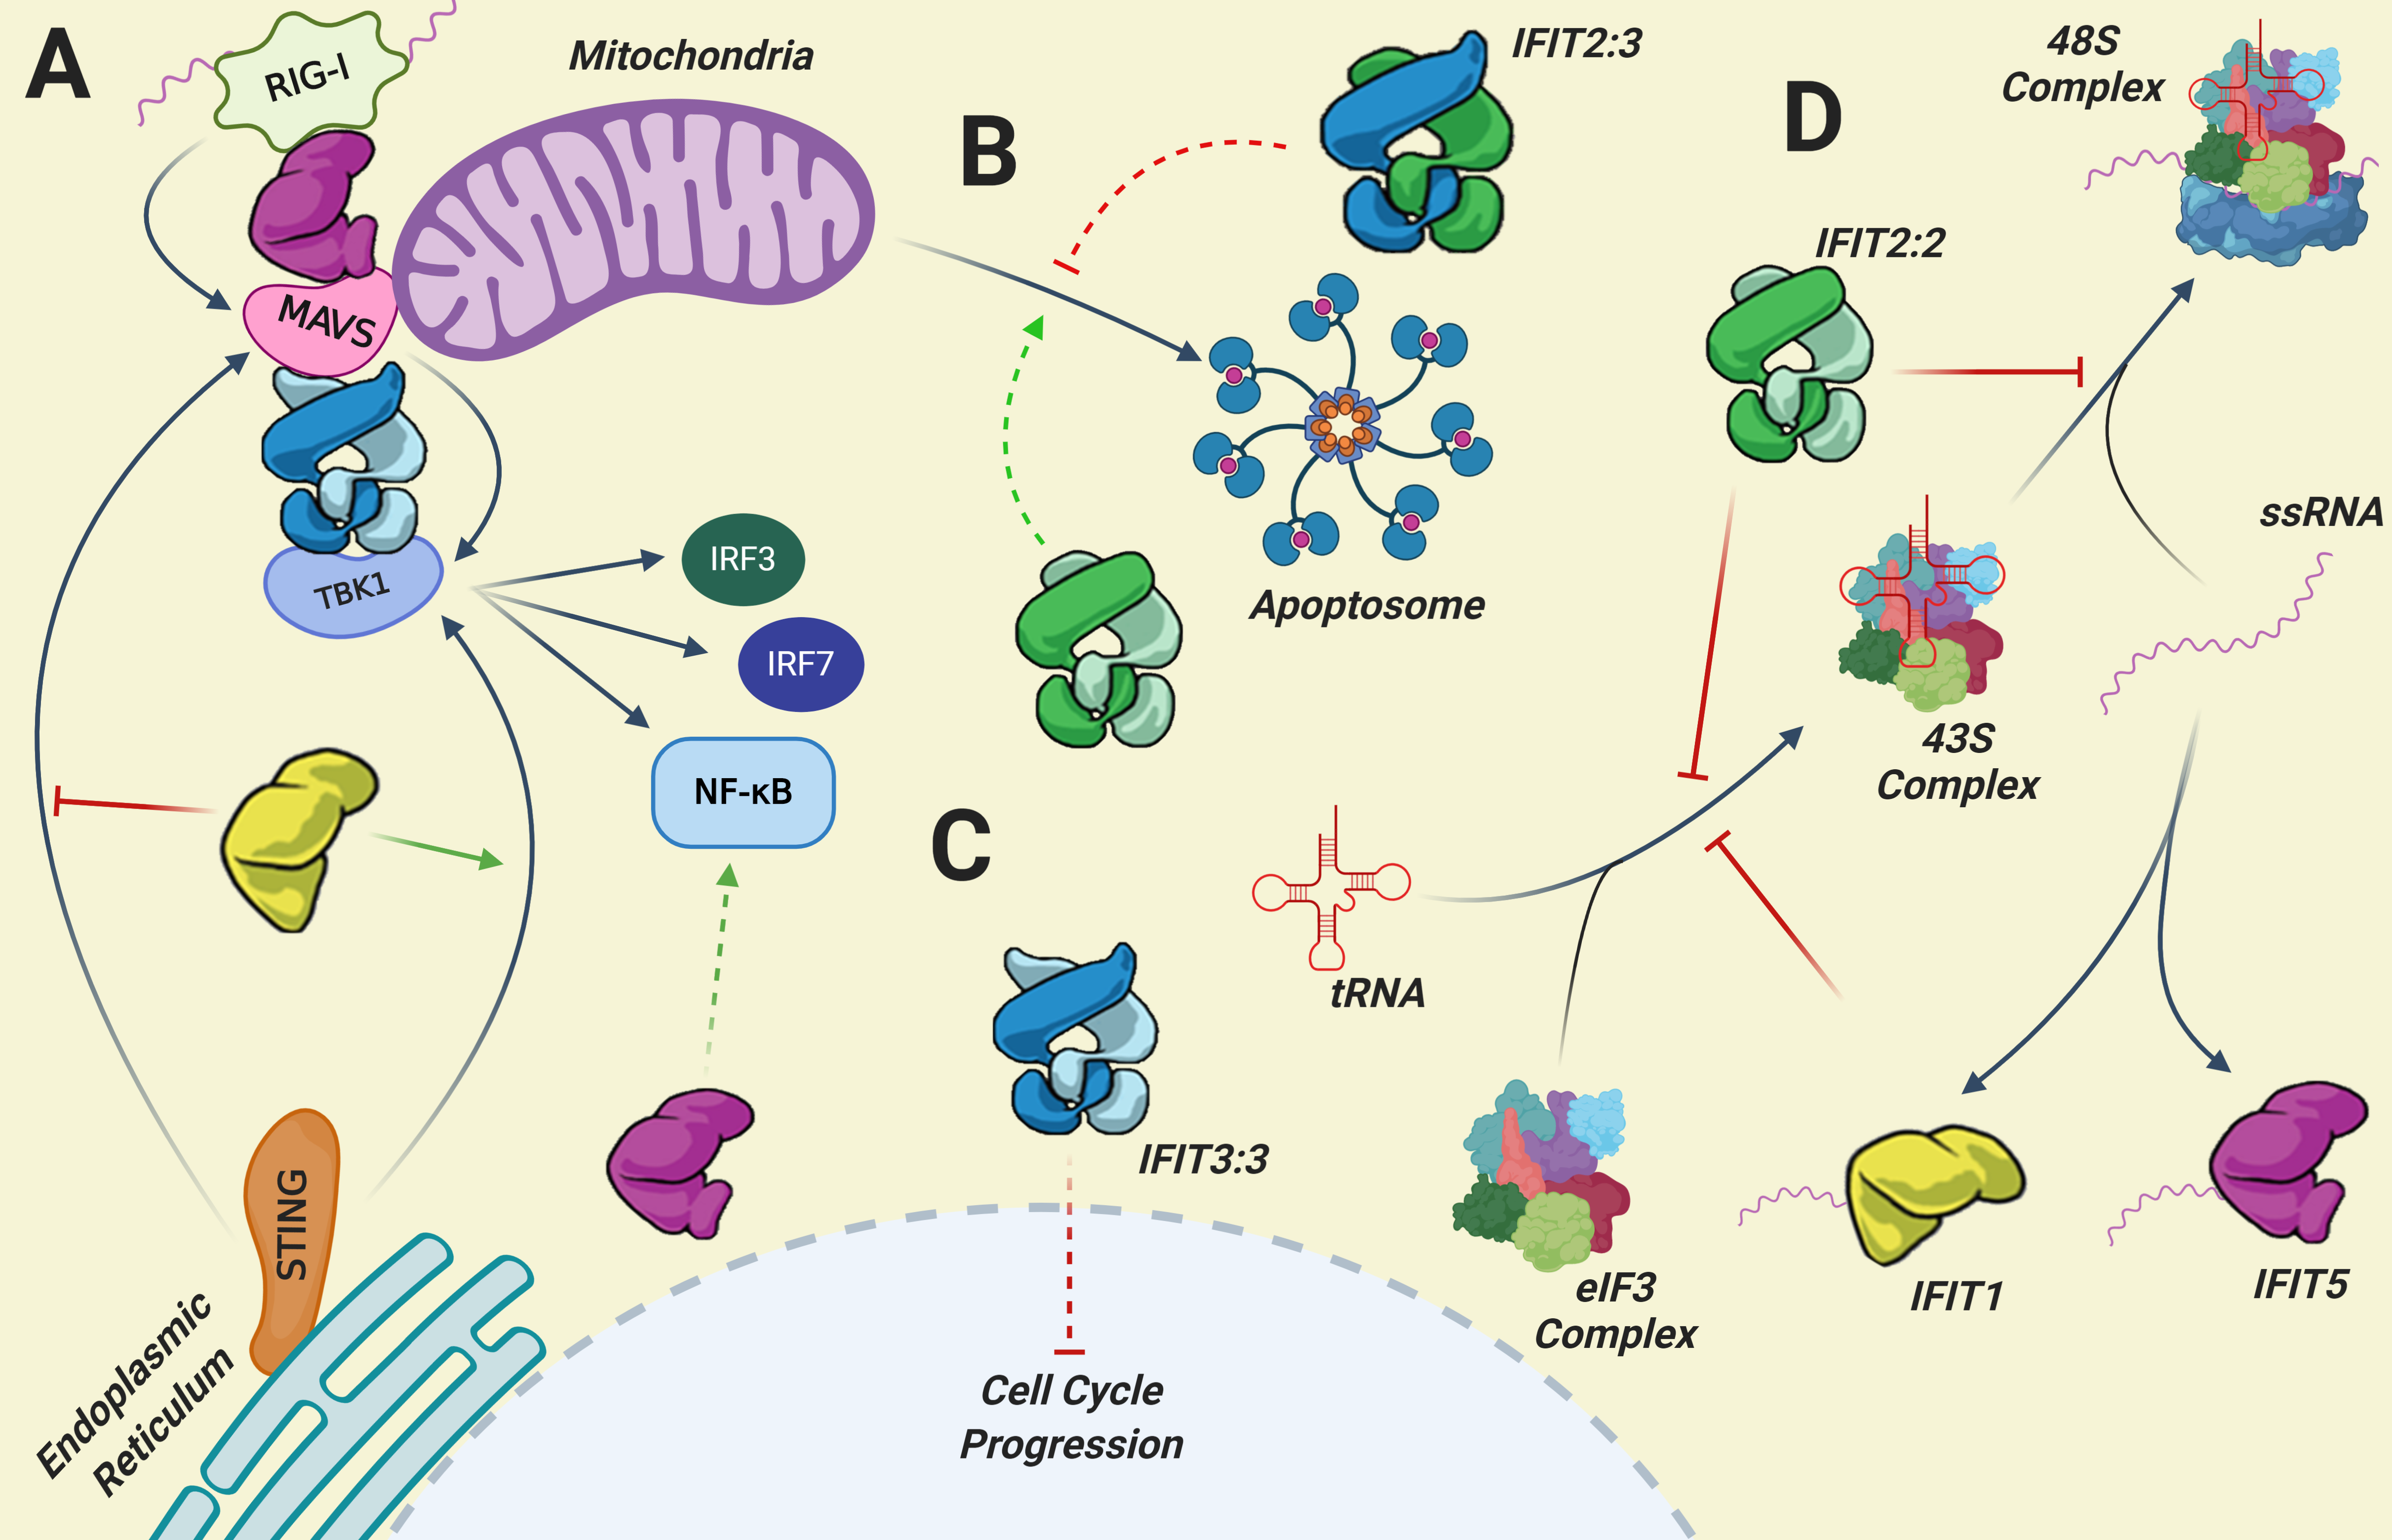
\includegraphics[width=1\linewidth]{04. Introduction//Figs/06. IFIT Mechanism of Action.png}
    \caption[Overview of IFIT Mechanisms of Action.]{\textbf{Overview of IFIT Mechanisms of Action.} IFITs have been described to have multiple actions in cells. Pathway A shows their involvement in innate immune signalling modulation. IFIT5 potentiate RIG-I activation of MAVS by scaffolding the two proteins together. IFIT3:3 further scaffolds MAVS to its effector, TBK1, which induces IRF3, IRF7 and NF\(\kappa\)B nuclear translocation when activated. STING protein also potentiates MAVS and TBK1 interaction. IFIT1 has been observed to inhibit STING interaction with MAVS while potentiating its interaction with TBK1. IFIT5 can also indirectly activate NF\(\kappa\)B. Pathway B shows IFIT2:2 involvement with apoptosome formation. IFIT2:3 complex reduces the pro-apoptotic activity of IFIT2:2. IFIT3:3 is involved in cell cycle arrest, as depicted in pathway C. Pathway D shows IFIT inhibition of viral replication and cellular translation. IFIT1 and IFIT5 can directly bind to cap0 and 5’PPP mRNA respectively and prevent its translation. IFIT1 and IFIT2 can both prevent 43S complex formation, while IFIT2 can also inhibit 48S complex formation. IFIT, Interferon-Induced Protein with Tetratricopeptide Repeats; RIG-I, retinoic acid-inducible gene I; MAVS, mitochondrial antiviral signalling protein; TBK1, TANK-binding kinase 1; STING, stimulator of interferon genes; IRF, interferon regulatory factor; NF\(\kappa\)B, nuclear factor kappa B; eIF, eukaryotic elongation factor; ssRNA, single-stranded RNA; tRNA, transfer RNA. The figure was adapted from \cite{Mears2018BetterResponse} and \cite{Diamond2013TheProteins}. Created using BioRender.com.}
    \label{fig:Overview of IFIT Mechanisms of Action}
\end{figure}




\subsection{IFIT During Cancer and Sepsis} \label{subsec:IFIT During Cancer and Sepsis}
ADD TEXT!! ADD TEXT!! ADD TEXT!! ADD TEXT!! ADD TEXT!! ADD TEXT!! ADD TEXT!! ADD TEXT!! ADD TEXT!! ADD TEXT!! ADD TEXT!! ADD TEXT!! ADD TEXT!! ADD TEXT!! ADD TEXT!! ADD TEXT!! ADD TEXT!! ADD TEXT!! ADD TEXT!! ADD TEXT!! ADD TEXT!! ADD TEXT!! ADD TEXT!! ADD TEXT!! ADD TEXT!! ADD TEXT!! ADD TEXT!! ADD TEXT!! ADD TEXT!! ADD TEXT!! ADD TEXT!! ADD TEXT!! ADD TEXT!! ADD TEXT!! ADD TEXT!! ADD TEXT!! ADD TEXT!! ADD TEXT!! ADD TEXT!! ADD TEXT!! ADD TEXT!! 




\subsection{IFIT Responses to Viral Infections} \label{subsec:IFIT Responses to Viral Infections}
\subsubsection{Human IFIT Responses to RNA Viruses} \label{Human IFIT Responses to RNA Viruses}
Human IFIT effects on single-stranded RNA viruses have been studied extensively within the past decade. \cite{Rabbani2016Identification3} reported that IFIT1 and IFIT3 restrict human parainfluenza virus 3 (PIV3, negative-sense ssRNA virus), while ectopic expression of IFIT2 and IFIT5 did not affect the viral fitness. \textit{In vitro} IFIT1 knock-down experiments using short hairpin RNA showed marked enhancement of protein expression of human PIV2, PIV5, and mumps virus, all negative-sense ssRNA viruses (\cite{Andrejeva2013ISG56/IFIT1Synthesis}; \cite{Young2016HumanFamily}). Hantaviruses, a family of negative-sense ssRNA viruses such as Prospect Hill virus (PHV), and Tula virus (TULV), strongly induce IFIT3 expression during the course of their infection (\cite{Matthys2011TheInduction}). Another negative-sense ssRNA virus, which bears a segmented genome, influenza A virus, has been shown to upregulate IFIT1, IFIT2, and IFIT3 in primary macrophages during infection (\cite{Lietzen2011QuantitativeMacrophages}). Human IFIT1 has been observed to be differentially expressed during hepatitis C virus (HCV) infection. HCV was described to suppress IFIT1 upregulation and subsequent experiments showed an inverse relationship between artificial levels of IFIT1 and HCV ability to infect host cells (\cite{Raychoudhuri2011ISG56Replication}).




\subsubsection{Livestock IFIT Responses to Viral Infections} \label{Livestock IFIT Responses to Viral Infections}
Data on livestock IFIT responses to viral infections is currently limited. Bovine viral diarrhoea virus (BVDV), a positive-sense ssRNA virus has been shown to inhibit IFIT1 and IFIT3 expression in bovine endometrium, compared to IFN Tau treatment, however, levels of IFIT2 and IFIT5 were not assessed (\cite{Cheng2017AcuteEndometrium}). Segmented dsRNA virus Blue tongue 16 has been shown to induce both sheep and goat IFIT1, IFIT2, and IFIT3 proteins in peripheral mononuclear cells, although the level of induction and induction dynamics varied between the species. Although sheep and goat IFIT proteins exhibit high interspecies IFIT protein similarity (97-99\% amino acid identity) their functional roles, binding partners, promoter activation, and structure may differ between them.  Lastly, porcine reproductive and respiratory syndrome virus was shown to activate IFIT1 and IFIT3 in porcine alveolar macrophages and IFIT1 and IFIT5 in the lung. This further shows that IFIT responses are dependent on cell type and the tissue of origin (\cite{Xiao2010AberrantProfiling}; \cite{Zhou2011MolecularVivo/i}). As presented above, it is clear that there is an abundance of human IFIT response data with regards to RNA viruses, however, there is a need to better define livestock IFIT responses.




\subsection{Comparison between human and bovine} \label{subsec:Comparison between human and bovine}
Strucural comparison \newline 
Genomic comparison




\section{Respiratory Syncytial Virus} \label{sec:Respiratory Syncytial Virus}
Human and bovine respiratory syncytial virus (RSV) cause acute respiratory illness in their respective host species and thus cause a large economic burden for the healthcare system and livestock industry alike (\cite{Jha2016RespiratoryVirus}; \cite{Sacco2014RespiratoryCattle}). To date, there is a limited knowledge of how IFITs impact on the replication of RSV. 

Bovine and human RSV are enveloped viruses possessing negative-sense ssRNA genome approximately 15 kilobase-pairs in size. Upon viral attachment and entry, the genome is released into the cytoplasm in the form of a ribonucleoprotein i.e. a complex of RSV genome with its nucleoprotein (N protein) (\cite{Noton2015InitiationReplication}). Viral replication also requires the RNA-dependent RNA polymerase (L protein) and the phosphoprotein (P protein), whereas RSV transcription also requires M2-1 protein, which is hypothesised to prevent premature termination of this process (\cite{Tanner2014CrystalPhosphorylation}). RSV transcripts are modified with 5’ cap structures prior to their translation. Both viral replication and transcription were previously believed to happen diffusely throughout the cytoplasm; however, recent studies suggest viral inclusion bodies (IBs) are the main site for RSV replication and transcription (\cite{Rincheval2017FunctionalVirus}). 




\subsection{Disease} \label{subsec:Disease}
dfasdfasdf




\subsection{Composition} \label{subsec:Composition}
asdfasdf




\subsection{Life Cycle} \label{subsec:Life Cycle}
asdfasdf

\begin{figure}
    \centering
    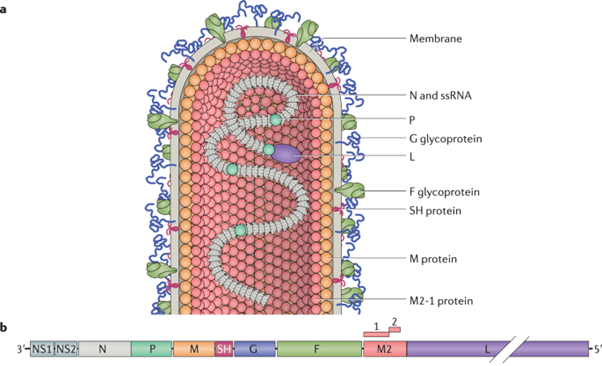
\includegraphics[width=0.5\linewidth]{04. Introduction//Figs/07. RSV-composition.png}

    
\end{figure}

\begin{figure}
    \centering
    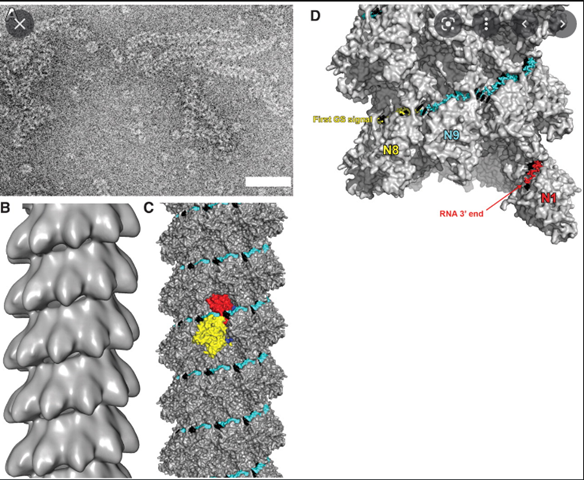
\includegraphics[width=0.5\linewidth]{04. Introduction//Figs/08. N-structure.png}
    
    
\end{figure}

\begin{figure}
    \centering
    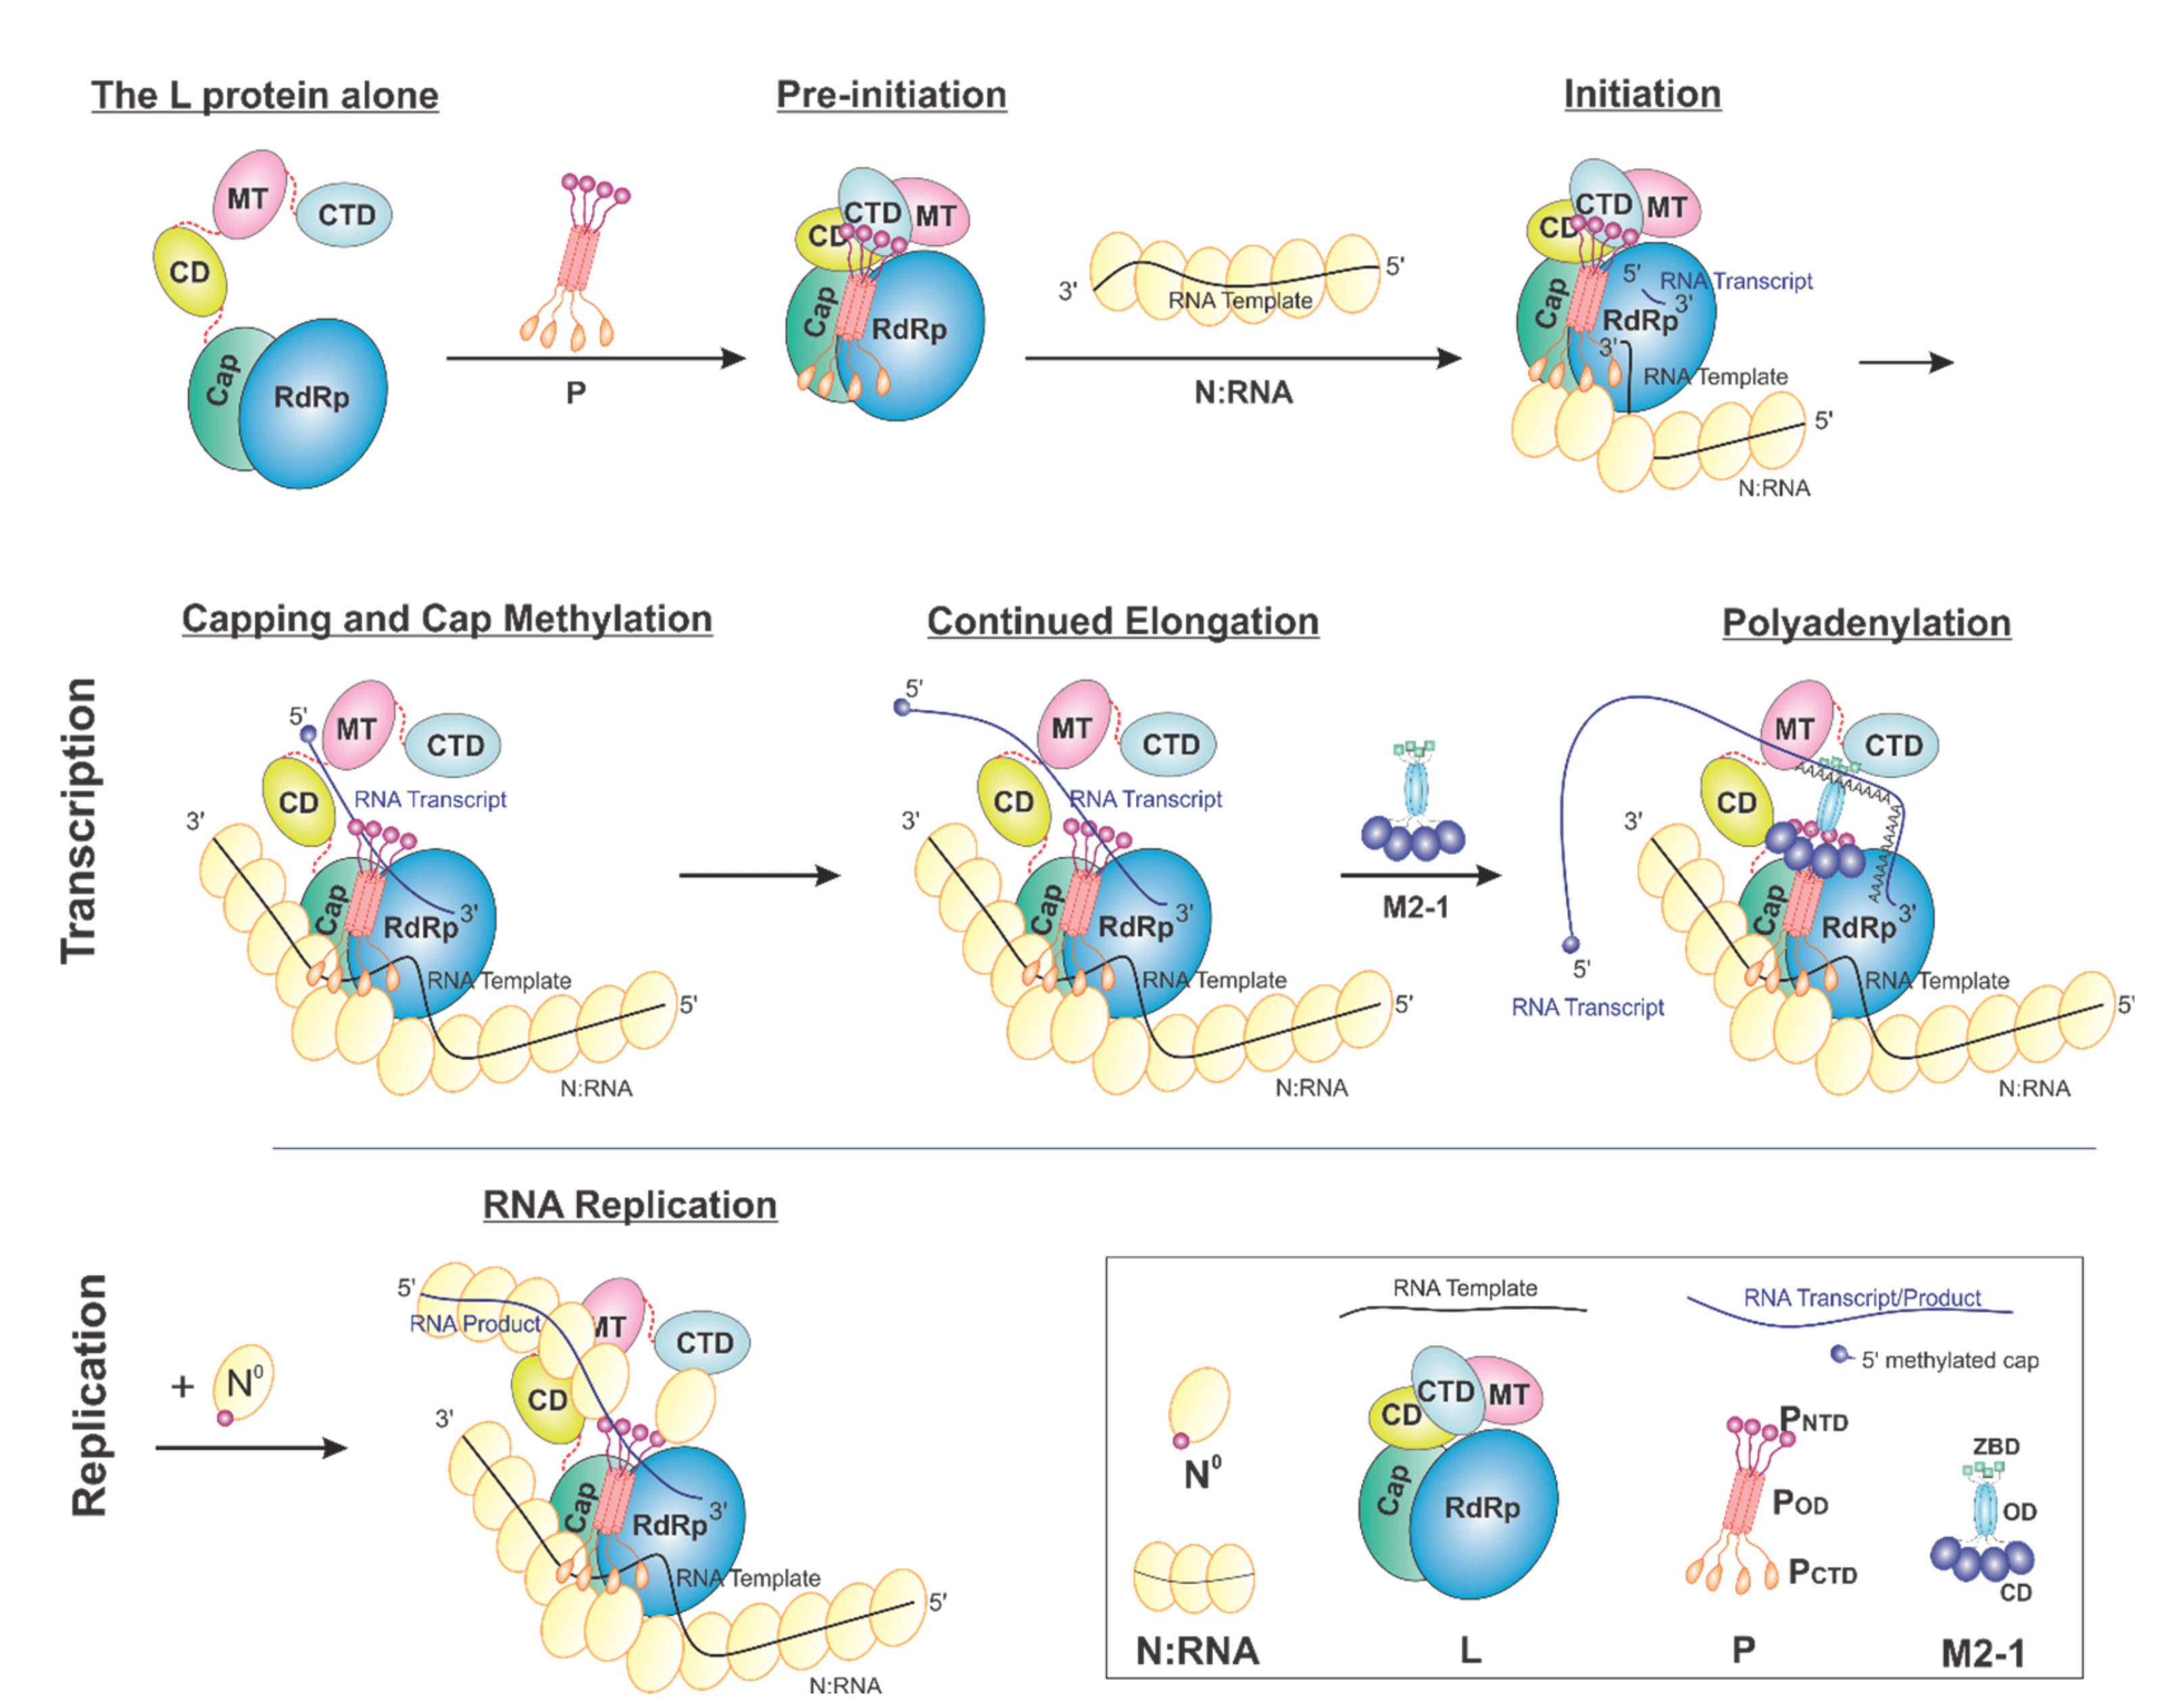
\includegraphics[width=0.5\linewidth]{04. Introduction//Figs/09. N_p_l_m21-interaction-overview.png}
    
    
\end{figure}

\begin{figure}
    \centering
    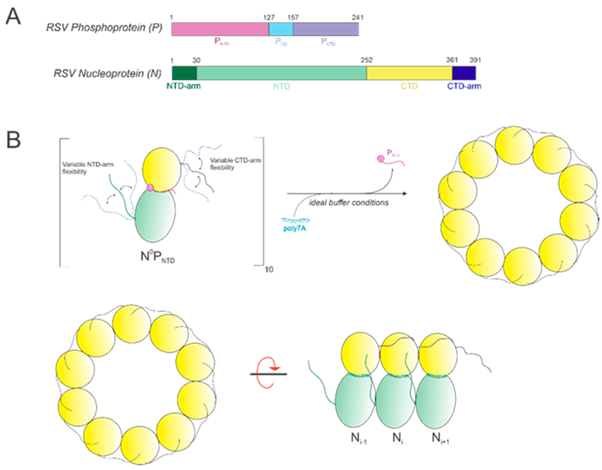
\includegraphics[width=0.5\linewidth]{04. Introduction//Figs/10. n-p interaction.png}
    
    
\end{figure}




\subsection{RSV Inclusion Bodies} \label{subsec:RSV Inclusion Bodies}
IBs are amorphous membranelles aggregates, which have been observed to form as early as 6 hours post-infection and often localise in close proximity to the nucleus (\cite{Bachi1973MorphogenesisVirus}; \cite{Jobe2020RespiratorySignaling}). They have characteristics of biomolecular condensates (with a similar electron density under electron microscopy to the nucleoli) and resemble cytoplasmic inclusions associated with other viral infections e.g. Negri bodies forming during rabies virus infection (\cite{Nikolic2017NegriOrganelles}). RSV N and P proteins are found on the edges of IBs, while L and M2-1 proteins are located inside the structure. (\cite{Rincheval2017FunctionalVirus}), using super-resolution imaging, discovered internal IB compartments called IB-associated granules (IBAGs). These not only contained different viral proteins compared to the rest of the IB, but nascent RNA labelling also suggested IBAGs to be the sites where newly synthesized mRNA concentrates (\cite{Jobe2020RespiratorySignaling}; \cite{Richard2018RSVTranscription}). Taken together, data suggests that IBs are specialised sites which enable viral replication and transcription and that these processes may be compartmentalised.

It is currently unknown if IFIT proteins interact with these structures. Given the well-described roles of IFITs in sensing viral RNA, it is possible that different IFITs may localise into IBs and IBAG, potentially interacting with viral RNA before the capping process takes place or directly interfere with the translational machinery. It is also possible that IFITs are restricted from accessing IBs by an unknown mechanism. Understanding these processes may reveal novel routes of increasing viral sensitivity to the innate immune response.




\subsubsection{Membrane-less Molecular Condensates and LLPS} \label{Membrane-less Molecular Condensates and LLPS}
ssdfasdfg



\subsubsection{IBAGs} \label{IBAGs}
asdfasdf



\subsubsection{Known Siphoning} \label{Known Siphoning}
asdfasdf



\subsection{Bovine vs Human Comparison} \label{subsec:Bovine vs Human Comparison}
asdfasdf




\section{Aims of the Study} \label{sec:Aims}
Here have a paragraph of the aims.

A detailed comparative study of human and bovine IFITs and their interaction with RSV. Looking at their induction, expression, and changes in localisation. Looking at interaction with RSV IBs. Assessing the involvement of IFIT2 in the RSV life cycle.

For your Aims make sure these are very detailed, so 2 pages roughly. Not 3-4 bullet points of 2 lines each, which I have seen!

%acronyms
\nomenclature[z-DEM]{DEM}{Untranslated}

\nomenclature[z-IBAG]{IBAG}{IB-Associated Granule}
\nomenclature[z-IB]{IB}{Inclusion Body}
\nomenclature[z-BVDV]{BVDV}{Bovine Viral Diarrhoea Virus}
\nomenclature[z-HCV]{HCV}{Hepatitis C Virus}
\nomenclature[z-TULV]{TULV}{Tula Virus}
\nomenclature[z-PHV]{PHV}{Prospect Hill Virus}
\nomenclature[z-PIV3]{PIV3}{Parainfluenza Virus 3}
\nomenclature[z-STING]{STING}{Stimulator of Interferon Genes}
\nomenclature[z-TBK1]{TBK1}{TANK-Binding Kinase 1}
\nomenclature[z-HEK]{HEK}{Human Embryonic Kidney}
\nomenclature[z-eIF]{eIF}{Eukaryotic Initiation Factor}
\nomenclature[z-ssRNA]{ssRNA}{Single-Stranded RNA}
\nomenclature[z-TPR]{TPR}{Tetratricopeptide Repeat}
\nomenclature[z-IFIT]{IFIT}{Interferon-Induced Protein with Tetratricopeptide Repeats}
\nomenclature[z-ISG]{ISG}{interferon-Stimulated Gene}
\nomenclature[z-UTR]{UTR}{Untranslated Region}
\nomenclature[z-IRSE]{IRSE}{Interferon-Stimulated Response Elements}
\nomenclature[z-STAT]{STAT}{Signal Transducer and Activator of Transcription}
\nomenclature[z-JAK]{JAK}{Janus Kinase}
\nomenclature[z-IRF]{IRF}{Interferon Regulatory Factor}
\nomenclature[z-ISGF3]{ISGF3}{Interferon-Stimulated Gene Factor 3}
\nomenclature[z-5’-PPP]{5’-PPP}{5’-triphosphoate}
\nomenclature[z-m7G]{m7G}{7-methyl guanosine}
\nomenclature[z-dsRNA]{dsRNA}{Double-Stranded RNA}
\nomenclature[z-MAVS]{MAVS}{Mitochondrial Antiviral Signalling Protein}
\nomenclature[z-RIG-I]{RIG-I}{Retinoic Acid-Inducible Gene I}
\nomenclature[z-MDA5]{MDA5}{Melanoma Differentiation-Associated Gene 5}
\nomenclature[z-NF\(\kappa\)B]{NF\(\kappa\)B}{Nuclear Factor kappa B}
\nomenclature[z-RSV]{RSV}{Respiratory Syncytial Virus}
\nomenclature[z-PRR]{PRR}{Pattern Recognition Receptor}
\nomenclature[z-PAMP]{PAMP}{Pathogen-Associated Molecular Pattern}
\nomenclature[z-LPS]{LPS}{Lipopolysaccharide}
\nomenclature[z-TLR]{TLR}{Toll-Like Receptor}


